\section{Konzepterarbeitung}

\subsection{Morphologischer Kasten}

\begin{figure}[H]
    \begin{center}
    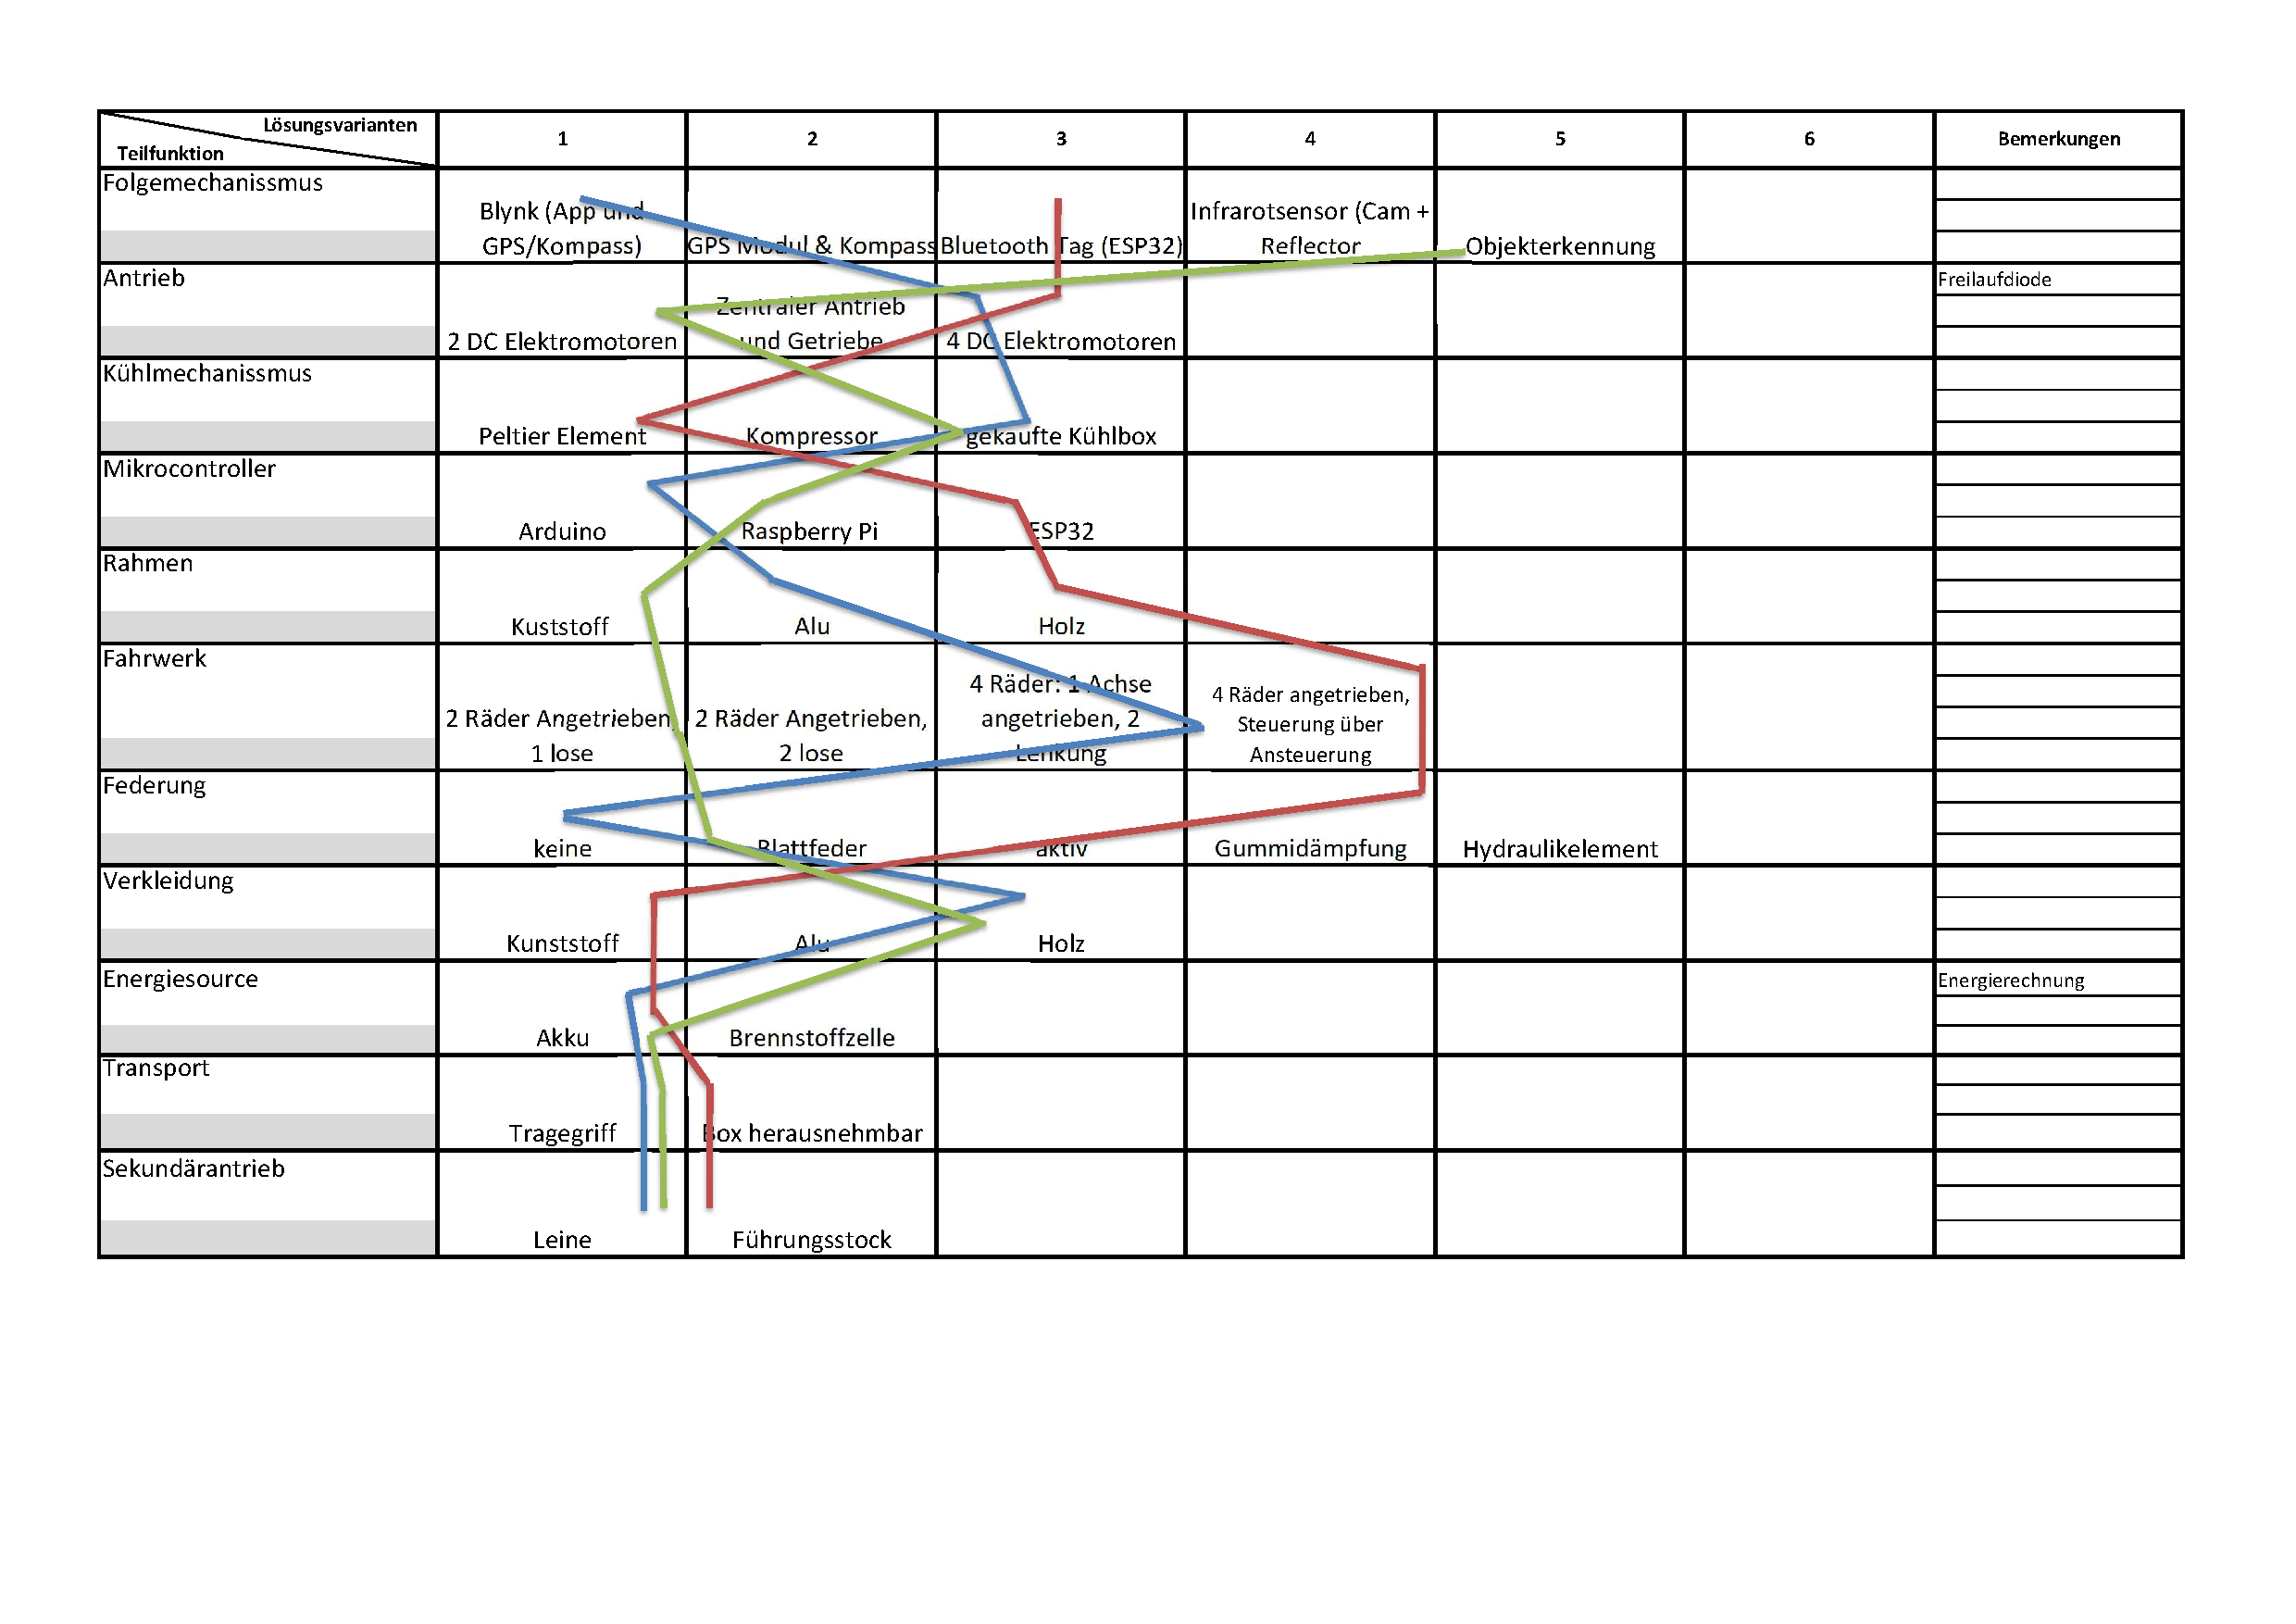
\includegraphics[width=\linewidth]{morph-kasten.pdf}
    \end{center}
    \caption{Morphologischer Kasten}
\end{figure}

Im morphologischen Kasten wurden drei verschiedene Lösungsvarianten für das Projekt eingetragen. Nach Abwägung der Schwierigkeit in der Herstellung und der Zuverlässigkeit in der Bedienung mithilfe des Zielkatalogs, wurde die blaue Lösung weiterverfolgt.

\subsection{Ressourcen Personell und Materiell}
Als intellektuelle Ressourcen gelten die Vorkenntnisse von Matthias Gass als Automatiker, Max Knauber als Motorradmechaniker und Fabian Schenker als Polymechaniker, wodurch die mechanische Seite des Projekts gut abgedeckt ist. Die Seite der Informatik bedarf etwas Einarbeitung, aber dank des bereits absolvierten Teils des Studiums der Mechatronik trinational gibts es auch dort einige Vorkenntnisse. \\
\\
Für technische Ressourcen und Fertigung von Kleinteilen seien folgende Werkstätten erwähnt:
\begin{itemize}
    \item 3D-Drucker
    \item Trinat-Labor
    \item Mechanische Werkstatt der FHNW-Muttenz
\end{itemize}

\subsection{Projektablauf}
In der folgenden Tabelle wird der Ablauf des Projekts inklusive Terminierung der Arbeitsschritte beschrieben.

\begin{table}[H]
    \centering
    \caption{Projektablauf}
    \label{tab:Projektablauf}
    \begin{tabular}{|ll|}
    \hline
    \rowcolor[HTML]{E0E0E0} 
    \multicolumn{2}{|l|}{\cellcolor[HTML]{E0E0E0}\textbf{Vorbereitungsphase}}                               \\ \hline
    \multicolumn{1}{|l|}{Grobkonzept erarbeiten}                                      & bis 21.10.2022      \\ \hline
    \multicolumn{1}{|l|}{\textbf{Freigabe Pflichtenheft}}                             & \textbf{21.10.2022} \\ \hline
    \rowcolor[HTML]{E0E0E0} 
    \multicolumn{2}{|l|}{\cellcolor[HTML]{E0E0E0}\textbf{Erster Prototyp}}                                  \\ \hline
    \multicolumn{1}{|l|}{Design erstellen}                                            & bis 18.11.2022      \\ \hline
    \multicolumn{1}{|l|}{Nötiges Material bestellen/erstellen}                        & bis 18.11.2022      \\ \hline
    \multicolumn{1}{|l|}{Erste mechanische Tests}                                     & bis 18.11.2022      \\ \hline
    \multicolumn{1}{|l|}{Erste Tests mit Elektronikkomponenten}                       & bis 18.11.2022      \\ \hline
    \multicolumn{1}{|l|}{\textbf{Meeting mit Stakeholder}}                            & \textbf{18.11.2022} \\ \hline
    \rowcolor[HTML]{E0E0E0} 
    \multicolumn{2}{|l|}{\cellcolor[HTML]{E0E0E0}\textbf{Zweiter Prototyp}}                                 \\ \hline
    \multicolumn{1}{|l|}{Design verbessern}                                           & bis 16.12.2022      \\ \hline
    \multicolumn{1}{|l|}{Weitere mechanische Tests}                                   & bis 16.12.2022      \\ \hline
    \multicolumn{1}{|l|}{Kühlbox anpassen}                                            & bis 16.12.2022      \\ \hline
    \multicolumn{1}{|l|}{\textbf{Meeting mit Stakeholder}}                            & \textbf{16.12.2022} \\ \hline
    \rowcolor[HTML]{D9D9D9} 
    \multicolumn{2}{|l|}{\cellcolor[HTML]{D9D9D9}\textbf{Finales Design}}                                   \\ \hline
    \multicolumn{1}{|l|}{Finales Design}                                              & 30.12.2022          \\ \hline
    \multicolumn{1}{|l|}{Elektrik verlegt und angeschlossen}                          & 30.12.2022          \\ \hline
    \multicolumn{1}{|l|}{Software einsatzbereit}                                      & 30.12.2022          \\ \hline
    \multicolumn{1}{|l|}{Voraussichtliche Beendigung}                                 & 08.01.2023          \\ \hline
    \rowcolor[HTML]{D9D9D9} 
    \multicolumn{1}{|l|}{\cellcolor[HTML]{D9D9D9}\textbf{Präsentation und Bewertung}} & \textbf{10.01.2023} \\ \hline
    \end{tabular}
    \end{table}

\subsection{Grobschätzung des Aufwands}
Der Aufwand, in Stunden, wurde in der untenstehenden Tabelle grob geschätzt und pro Person aufgeteilt.

\begin{table}[H]
    \centering
    \caption{Grobschätzung des Aufwands}
    \label{tab:Aufwand}
    \begin{tabular}{|l|l|l|l|}
    \hline
    \textbf{Thematik}         & \textbf{Matthias} & \textbf{Max} & \textbf{Fabian} \\ \hline
    Grundkonzept   erarbeiten & 4                 & 4            & 4               \\ \hline
    Pflichtenheft             & 4                 & 8            & 4               \\ \hline
    Materialbeschaffung       & 3                 & 4            & 2               \\ \hline
    Erster   Prototyp         & 2                 & 2            & 30              \\ \hline
    Zweiter   Prototyp        & -                 & 4            & 25              \\ \hline
    Finales   Design          & 16                & 16           & 8               \\ \hline
    Kühlbox-Umbau             & 12                & -            & -               \\ \hline
    Elektronik   verkabeln    & 8                 & 6            & -               \\ \hline
    Software                  & -                 & 60           & 10              \\ \hline
    Dokumentation             & 5                 & 6            & 10              \\ \hline
    Präsentation              & 2                 & 2            & 2               \\ \hline
    Testen                    & 6                 & 20           & 10              \\ \hline
    Video                     & 25                & 1            & 1               \\ \hline
    \textbf{Total}            & \textbf{87}       & \textbf{133} & \textbf{106}    \\ \hline
    \end{tabular}
    \end{table}

    \pagebreak

\subsection{Budget}

\begin{table}[H]
    \centering
    \caption{Budget (maximal 200.00 CHF)}
    \label{tab:Budget}
    \resizebox{\textwidth}{!}{%
    \begin{tabular}{|l|l|l|l|l|}
    \hline
    \rowcolor[HTML]{009999} 
    \textbf{Gegenstand}                & \textbf{Rechnung (in CHF)} & \textbf{Datum   Rechnung} & \textbf{Lieferant}  & \textbf{Rechnungsnummer} \\ \hline
    Bollerwagen -   Räder              & 20.00                      & 10.10.2022                & Tutti               & 1                         \\ \hline
    Kühlbox   elektrisch               & 20.00                      & 20.10.2022                & Tutti               & 2                         \\ \hline
    GPS Modul: Zhiting Neo 7m          & 11.73                      & 24.10.2022                & Amazon              & 3                         \\ \hline
    Bluethooth   Modul: HC-06          & 8.78                       & 24.10.2022                & Amazon              & 3                         \\ \hline
    Kompass   Modul: AZDelivery GY-271 & 6.21                       & 24.10.2022                & Amazon              & 3                         \\ \hline
    2Pcs   Schrittmotortreiber BTS7960 & 15.77                      & 24.10.2022                & Amazon              & 3                         \\ \hline
    Spannungsregler:   LM2596HV        & 6.90                       & 24.10.2022                & Amazon              & 3                         \\ \hline
    Zylinderschrauben   lang M6x60     & 11.74                      & 15.11.2022                & Hornbach            & 4                         \\ \hline
    Sechskantschraube   M8x140         & 3.90                       & 15.11.2022                & Obi                 & 5                         \\ \hline
    Step-Up   12-35V 150W              & 8.86                       & 18.11.2022                & Amazon              & 6                         \\ \hline
    Deans T-Plug   Steckverbindungen   & 7.55                       & 18.11.2022                & Amazon              & 6                         \\ \hline
    Transport   Lenkrolle 125mm 100kg  & 10.60                      & 03.12.2022                & Galaxus             & 7                         \\ \hline
    Rundrohr Alu                       & 6.10                       & 31.12.2022                & Jumbo               & 8                         \\ \hline
    Holzzuschnitt                      & 9.05                       & 20.12.2022                & Jumbo               & 9                         \\ \hline
                                       &                            &                           &                     &                           \\ \hline
    PLA/PET Teile   gedruckt           & 52.80                      &                           & Fabian/Max/Matthias & 99                        \\ \hline
                                       &                            &                           &                     &                           \\ \hline
    Batterie:                          &                            & Gestellt von der FHNW     & FHNW                & 0                         \\ \hline
    Arduino:                           &                            & Gestellt von der FHNW     & FHNW                & 0                         \\ \hline
                                       &                            &                           & Fabian              &                           \\ \hline
    Motoren:                           &                            & Gestellt von Fabian       &                     & 0                         \\ \hline
    Holzreste:                         &                            & Gestellt von Matthias     & Matthias            & 0                         \\ \hline
    \rowcolor[HTML]{C6E0B4} 
    \textbf{Gesamte   Rückzahlung}     & \textbf{199.99}            & \textbf{}                 & \textbf{}           & \textbf{}                 \\ \hline
    \end{tabular}%
    }
    \end{table}